\chapter{基于 TLA+ 的 OT函数验证} 
\section{TLA+ 简介}
\par TLA+是一种形式化的规约语言。它是一种设计系统和算法的工具,并且用来验证这些系统有没有关键错误。
\par 正确性,是一个系统最为重要的性质,同时,正确性是比较难以证明的,特别是并发系统的正确性,因为存在着数目众多的状态变化,而TLA+可以将系统的行为或者状态抽象为时态逻辑,即系统的行为或者状态会随着时间反生变化,然后通过一些数学分析的方法,来判断系统是否正确。

TLA+ model checker 与经典的模型检验工具类似,通过遍历系统模型的所有可能的行为,验证其正确性。

\par TLA+并不同于一般传统意义上的编程语言,更类似于一种数学语言,因为其语法大部分来自于实际的数理逻辑。
\par TLA+提供了工具集TLAToolbox/TLC,同时还可以使用TLA+的语法糖PLUSCAL来完成代码的编写,由于本文中并未涉及,在此不做展开。

figure: assume 删除; 英文注释; 类似宏 删除; 空行

\begin{figure}
\centering
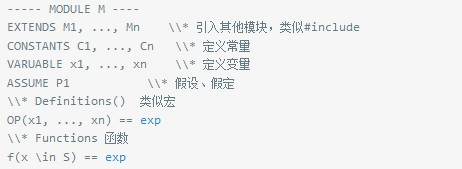
\includegraphics{figures/module.jpg}
\caption{TLA+编码模板}
\label{fig:graph}
\end{figure}

\subsection{TLA+ Modules}
TLA+ 提供了多种数据结构的实现,包括 $\dots$。

record

在本次实验中,我们引入了TLA+ 中的Sequences模块,将List表示为一个Sequecnce,并且使用了如下的API:\\
\begin{tabular}{ccc}
\hline
operator& operation& example \\
\hline  
 Head& First element &Head(<<1, 2>>) = 1\\
 Tail& Sequence aside from head &Tail(<<1, 2>>) = <<2>>\\
 Append& Add element to end of sequence &Append(<<1>>, 2) = <<1, 2>>\\ 
 Len& Length of sequence &Len(<<1, 2>>) = 2\\
\hline % 
\end{tabular}

\section{使用 TLA+ 描述 OT 函数}

解释同时描述并验证第一类和第二类 OT 函数。
 	 	
\subsection{OT函数设计}
\subsubsection{第一、二类函数的表示}
数据结构: 操作的表示 (record)

代码示例 (ins vs. del)

\subsubsection{第三、四类函数的表示}
如何生成区间?

如何递归?

代码示例

\subsubsection{命令执行的表示}

\section{正确性验证}

验证的目标: CP1 如何用 TLA+ 表示。

\par 我们验证CP1性质的正确性。即同一个List经过OT(OP2,OP1),OP1或者OT(OP1,OP2),OP1这两种操作序列后,最终的结果是一致的。
\par 用TLA+来描述就是:
\begin{align*}
  apply(apply(list,op1),Xform(op2, op1)) = apply(apply(list,op2),Xform(op1, op2))
\end{align*}
\par 只要对于任意的两个操作,这个等式都成立的话,那么CP1正确性即可得到验证。

没有 Init 和 Next, 采用 ``Evaluate Constant Expression'' (TLA+ 有这种功能)


如何利用 TLA+ 的遍历的能力。

\subsection{TLA+ Model Checker 设置}


常量定义 (确定除list之外的参数值)

core 数目

\subsection{实验结果}

三张图,每张图变换list的长度 (1,3,5,7,9,15,20,25,30,40,50,60,80,100,150,200),记录验证所需的时间。

pgfplots